% !TeX TS-program = pdflatex
% !BIB TS-program = biber
% !TeX encoding = UTF-8
% !TeX spellcheck = it_IT
% !TeX root = calcolatrici.tex
\documentclass[a4paper,oneside]{book}%
% 21/01/2018 :: 22:12:46 :: \documentclass{book}%
\usepackage{cmap}
\frenchspacing%
\usepackage{base}
\usepackage[big]{layaureo}
\usepackage{grafica}
\usepackage{stand_class}
\usepackage{matematica}
\usepackage{tabelle}
\usepackage{date}
\usepackage{pagina}
\usepackage{unita_misura}
\usepackage{utili}
\usepackage{copyright}
\usepackage{CDloghi}
\newcommand{\HRule}{\rule{\linewidth}{0.5mm}}

\usepackage[grumpy,mark,markifdirty,raisemark=0.95\paperheight]{gitinfo2}  
\usepackage[toc,page]{appendix}
\renewcommand{\appendixtocname}{Appendici}
\renewcommand{\appendixpagename}{Appendici}
\usepackage{imakeidx}
\makeindex[options=-s ../Mod_base/oldclaudio.sti]

\usepackage[style=italian]{csquotes}
\usepackage[%
style=philosophy-modern,
annotation=true,
hyperref,
backend=biber,
backref]{biblatex}
\addbibresource{calcolatrici.bib}
\usepackage[italian]{varioref}
\usepackage{hyperxmp}
\usepackage[pdfpagelabels,plainpages=false]{hyperref}
\usepackage[italian]{cleveref}
\title{Calcolatrici}
\author{Claudio Duchi}
\date{\datetime}
\hypersetup{%
	pdfencoding=auto,
	urlcolor={blue},
	pdftitle={Calcolatrici},
	pdfsubject={Calcolatrici},
	pdfstartview={FitH},
	pdfpagemode={UseOutlines},
	pdflicenseurl={http://creativecommons.org/licenses/by-nc-nd/3.0/},
	pdflang={it},
	pdfmetalang={it},
	pdfkeywords={Calcolatrici},
	pdfcopyright={Copyright (C) 2021, Claudio Duchi},
	pdfcontacturl={http://breviariomatematico.altervista.org},
	pdfcontactpostcode={06128},
	pdfcontactphone={},
	pdfcontactemail={claduc},
	pdfcontactcountry={Italy},
	pdfcontactcity={Perugia},
	pdfcontactaddress={},
	pdfcaptionwriter={Claudio Duchi},
	pdfauthortitle={},%
	pdfauthor={Claudio Duchi},
	linkcolor={blue},
	colorlinks=true,
	citecolor={red},
	breaklinks,
	bookmarksopen,
	verbose,
	baseurl={http://breviariomatematico.altervista.org}
}
%\usepackage[acronyms,translate=false,nonumberlist,toc,numberedsection,counter=chapter,automake]{glossaries-extra}
%\usepackage{glossary-mcols}
%\usepackage{glossary-longragged}
%\usepackage{glossaries-babel}
%\makeglossaries
%\renewcommand*{\glsxtrpostdescgeneral}{%
%	\ifglshasfield{see}{\glscurrententrylabel}
%	{, \glsxtrusesee{\glscurrententrylabel}}%
%	{}%
%}
%\setglossarystyle{altlistgroup}
%\loadglsentries{glossari1}
\listfiles
\makeatletter
\renewcommand\frontmatter{%
	\cleardoublepage
	\@mainmatterfalse
	\pagenumbering{arabic}}
\renewcommand\mainmatter{%
	\cleardoublepage
	\@mainmattertrue}
\makeatother
\includeonly{copy,offixe,kadio,maxexcell,sharp}
\setkeys{Gin}{width=.75\textwidth}

\begin{document}
	\frontmatter
		\hypersetup{pageanchor=false}
		\begin{titlepage}\parindent=0pt
			\centering
	\begin{center}
	\Lgrandedue\\[1cm]
	\textsc{\LARGE Claudio Duchi}\\[1.2cm]
	\HRule \\[0.4cm]
	{ \huge \bfseries CALCOLATRICI}\\[0.4cm]
	\HRule \\[1.2cm]
	\vfill
	\polylogo[5.5]{15}		
	{\large $-$\DTMnow$-$}	
\end{center}
{\centering
	Release:\gitReln\ (\gitAbbrevHash)\ Autore:\gitAuthorName\ 
	\gitCommitterDate \\
}
		\end{titlepage}
	\setcounter{page}{2}
	Tutti marchi sono di proprietà dei rispettivi proprietari. 
		\CDcopyright
		\tableofcontents
		\listoffigures
		\listoftables
		\mainmatter
\chapter{OFFIXE}
\section{KD-82MS (Z171)}\index{OFFIXE!Z171}
Calcolatrice prodotta in Cina, probabile clone Casio FX-82MS\index{Casio!FX82MS}
\subsection{Test interno}
Il test\[\arcsin(\arccos(\arctan(\tan(\cos(\sin(9))))))=9\] ha come risulta dalla tabella~\vref{tab:OFFIXEKD82MS}. 
\subsection{Modi funzionamento}
La calcolatrice ha tre modi di funzionamento, calcoli aritmetici di base, deviazione standard, calcoli di regressione
\subsection{Formati visualizzazione}
\CASIOmodediplayexp

\begin{table}
	\centering
		\begin{tabular}{lll}
		\toprule
		\multicolumn{1}{c}{Modello}&\multicolumn{1}{c}{Risultato}&\multicolumn{1}{c}{Errore}\\
		\midrule
		OFFIXE KD-82MS(Z171)&\num{8.9999999998}&\num{1.921103e-9}\\
		\bottomrule
	\end{tabular} 
	\caption{OFFIXE KD-82MS (Z171)}
	\label{tab:OFFIXEKD82MS}
\end{table}
\begin{table}\centering
	\begin{tabular}{ccc}
	\toprule
	MODO	&TASTI  &  DISPLAY\\ 
		\midrule 
	Calcoli aritmetici di base	& \tastomode\tasto{1} & COMP \\ 
		\midrule 
	Deviazione standard	&\tastomode\tasto{2}  & SD \\ 
		\midrule 
	Calcoli di regressione	&\tastomode\tasto{3}  & REG  \\ 
		\bottomrule
	\end{tabular} 
		\caption{Modi: OFFIXE KD-82MS (Z171)}
	\label{tab:OFFIXEKD82MSModi}
\end{table}
\begin{figure}
	\begin{subfigure}[b]{.5\linewidth}
	\centering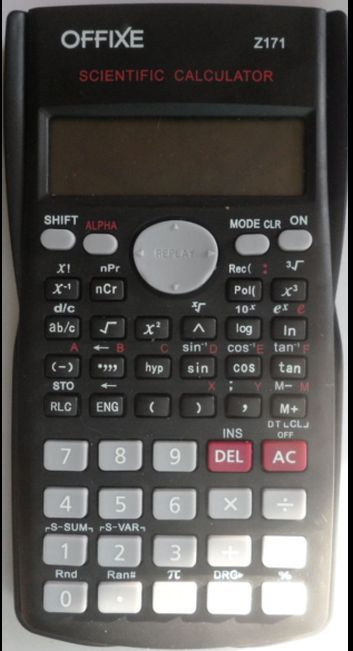
\includegraphics{offixe/SAM_3719}%
		\caption{Fronte}\label{fig:OFFIXEfront}
	\end{subfigure}%
	\begin{subfigure}[b]{.5\linewidth}
   \centering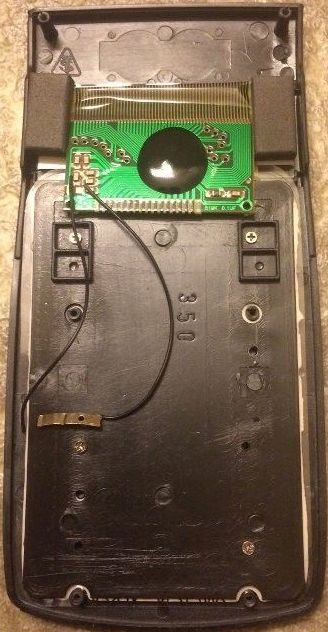
\includegraphics{offixe/7019561509344433257}%
		\caption{PCB}\label{fig:OFFIXEPCB}
	\end{subfigure}
	\caption{OFFIXE KD-82MS (Z171)}\label{fig:OFFIXEKD82MS}
\end{figure}
		
%\cleardoublepage
%\glsaddall	
%\twocolumn
%\printglossaries
%\onecolumn		
\nocite{*}
 \addcontentsline{toc}{chapter}{\bibname}
\printbibliography
\printindex
\backmatter
\appendix
\chapter{Mezzi usati}
\CDMezziUsati
\end{document}
